\documentclass[a4paper,10pt]{article}
\usepackage[toc,page]{appendix}
\usepackage[margin=2.5cm]{geometry}
\usepackage[utf8]{inputenc}
\usepackage{listings}
\usepackage{tikz}
\usepackage{forest}
\usepackage{textcomp}
\usepackage{url}
\usepackage{pdflscape}
\usepackage[nottoc,numbib]{tocbibind}

\lstset{language=Python,upquote=true} 

\usetikzlibrary{shapes.geometric, arrows, positioning, fit}

\tikzstyle{stepa} = [rectangle, rounded corners, minimum width=3cm, minimum height=1cm, text centered, text width=3cm, draw=black]

\tikzstyle{outcome} = [rectangle, dotted, minimum width=1cm, minimum height=1cm, text centered, text width=3cm, draw=black]

\tikzstyle{infosource} = [circle, minimum width=3cm, minimum height=1cm, text centered, text width=3cm, draw=black]

\tikzstyle{startstop} = [diamond, minimum width=3cm, minimum height=1cm, text centered, draw=black, fill=black!15]

\tikzstyle{phase} = [rectangle, dashed, draw=black]

\tikzstyle{arrow} = [thin,->,>=stealth]

%opening
\title{CITS5502: Assignment 1 -- Characteristics of a Software Process}
\author{Ash Tyndall, 20915779}

\begin{document}
\newgeometry{margin=3.2cm}
\maketitle
\tableofcontents

\clearpage

\section{Essay \& Conclusions}
\fontsize{11pt}{13pt}\selectfont
Software is everywhere. In the modern world, nearly everything is controlled by, managed by or was ultimately created by software. Modern software carries high expectations, thus it is in the interest of organisations who develop software to create and enforce processes that ensure that software is be developed free of bugs, to requirements, within a sensible timeframe.

However, software engineering is also a notorious industry to develop processes for: Due to the breakneck pace at which client demands, available tools and technological norms evolve, there are multiple competing views on the best way to ensure the goal of quality software released inexpensively and rapidly is achieved.

A whole industry has sprung up around software development methodologies; processes that guide a team through the process of developing software in a way that hopes to achieve these goals. However, because this methodology industry in part is a for-profit one, the effectiveness or novelty of a given new process can take the backseat to marketing and economic concerns.

This leads us to ask the question; ``how similar are different software processes?'' When a new process appears, it can be useful to frame it in terms of differences to existing processes, and if the process has no significant differences, it can be helpful to know this easily. Finding these differences, as it turns out, is no simple task: A cursory internet search for each of these processes will yield a diagram of some form explaining how the process operates, however frequently these diagrams invent their own notation, which serves to obscure the process from comparison with other processes. 

It is clear that if one wishes to compare these processes, one must first design a notation that can describe the core of their processes in a similar way. This was the first step in my task, which is discussed in section \ref{sec:processes}. My notation is relatively simple, but I believe it presents a good balance between complexity and an ability to represent the defining characteristics of different processes.

A key part of my notation is its brevity, which is partly enabled by the lack of defined decision nodes; a decision is instead represented by multiple paths leaving a given node on the graph, with labels on some or all of these exit paths. When there is an unlabelled path and other labelled paths, it is assumed that you will always follow the labelled path if you meet the criteria of the label, otherwise you will take the unlabelled path. 

Another important part of my notation is the broader phase marker. This dashed box surrounds different sections of a process to indicate either that this section of nodes is considered a broader stage of the process or that there is some form of loop between the nodes represented in the section. This is not strictly necessary, but is provided for visual clarity.

Finally, a part of my notation that is seen in some processes is the presence of a ``deliverable/artifact node'' that does not trace its way back to the ``Start'' node of the process. This is seen for instance with the ``Scrum'' model in subsection \ref{sec:scrum}. This situation indicates that the given process has a prerequisite that is expected will be fulfilled outside of the process scope. As different software processes have different scopes, it is useful in this way to represent how ``out of scope'' information interacts with the process.

Once these notations were completed for the ten existing software processes and my personal process, it was clear to see that the level of specification each process provides varies wildly, and seems to be only loosely correlated with its relationship to similar processes. For instance both Dynamic Systems Development Method (DSDM; subsection \ref{sec:dsdm}) and Scrum are both considered to be ``Agile'' processes, however the level of expression between their processes differs massively. 

This example highlights a broader understanding I achieved regarding processes; there is a clear spectrum of formality in processes that appears to transcend the ``genre'' of the process. While the Agile processes I investigated here generally lent towards the ``no formality'' end of the spectrum, DSDM demonstrated that it is not necessary for this to be the case. While DSDM has codified several more steps than Scrum, it still ensures that there are heavy amounts of iteration in the process stages, a core principle of Agile.

The most linear of the processes I described was that of the Team Software Process (subsection \ref{sec:tsp}), which appears to replace the concept of iteration with the presence of intense and numerous testing periods and post-mortems at each stage of the process. The most simple of the processes I described, in my opinion, was that of Scrum, which only had eight nodes, and a very simple iterative cycle of develop, meet, determine amount of development remaining, which was iterated over within a strict time-limit.

This notation exercise also highlighted the similarities between many processes that I chose to represent in my notation. For instance, broad similarly was found between my own personal process, and that of the Iterative Development Model, Rational Unified Process and Agile Unified Process. The differences between them and my own were primarily in that I lack a design prototype stage, and scope investigation is not emphasised in my  personal process.

The similarity between those processes and my own was also emphasised with the creation of my taxonomy for software processes (section \ref{sec:tax}.) I elected to create a decision tree style system, whereby questions are asked and answered yes or no, until only one process matches the set of answers provided. The development of this tree was an interesting exercise in of itself, as while the questions could easily split the processes into a variety of different trees, it was important to find the right combination of questions to maximally represent the differences between the processes on the tree in the minimum amount of questions. This required considering a variety of combinations, until I settled on the set that can be seen in the aforementioned section. 

The taxonomy also exemplified some of the primary defining differences between the processes that I chose. The two primary questions were ``Are requirements reevaluated throughout?'' and ``Is client feedback or acceptance part of evaluation?'' The answers to these questions split the processes into a group of five and two groups of 3, which clearly demonstrated the different approaches to requirements and feedback within the processes I investigated.

In conclusion, we can see that many software processes that hold themselves as being different may not necessarily be as innovative as previously thought. While it is an involved task to take the varying source materials describing these processes and convert them into a common notation, there are large benefits to doing so, as they allow us to more easily see how the processes relate, their relative complexities, and how encompassing the iterative aspects of these processes are. 

The taxonomy created also assisted in defining the differences between processes, and could be a useful tool in future, as it can be indefinitely extended with new questions to differentiate between new processes. Together, this notation and taxonomy form a useful set of tools to critically evaluate existing and new software processes, to determine their true innovation, and if that innovation is different enough to justify the cost of embracing them.

\fontsize{10pt}{12pt}\selectfont
\restoregeometry
\clearpage
\section{Processes Notation}
\label{sec:processes}

\subsection{Key}
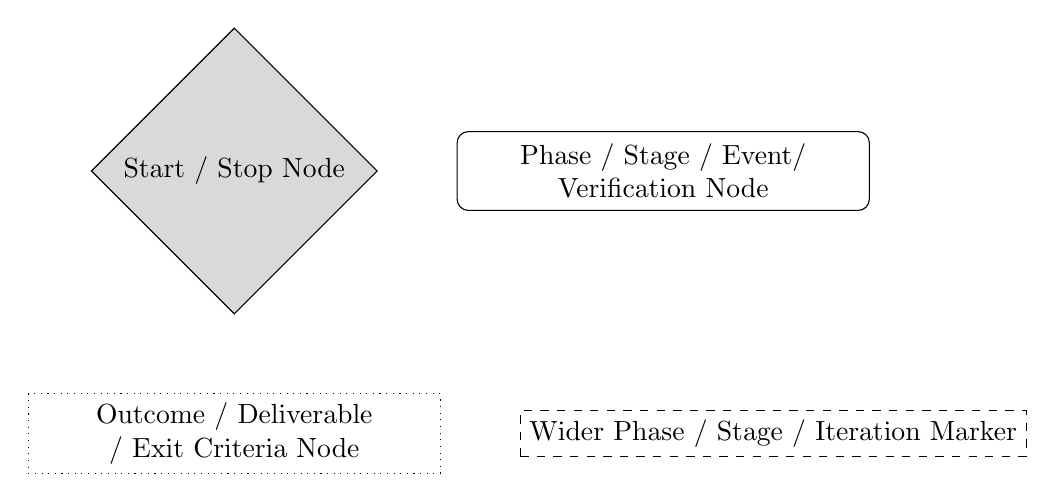
\begin{tikzpicture}[node distance=1cm]
 
 \node (startstop) [startstop] {Start / Stop Node};
 \node (stepa) [stepa, right=of startstop, text width=5cm] {Phase / Stage / Event/ Verification Node};
 \node (outcome) [outcome, below=of startstop, text width=5cm] {Outcome / Deliverable / Exit Criteria Node};
 \node (phase) [phase, right=of outcome] {Wider Phase / Stage / Iteration Marker};
\end{tikzpicture}

\subsection{Incremental Build Model}
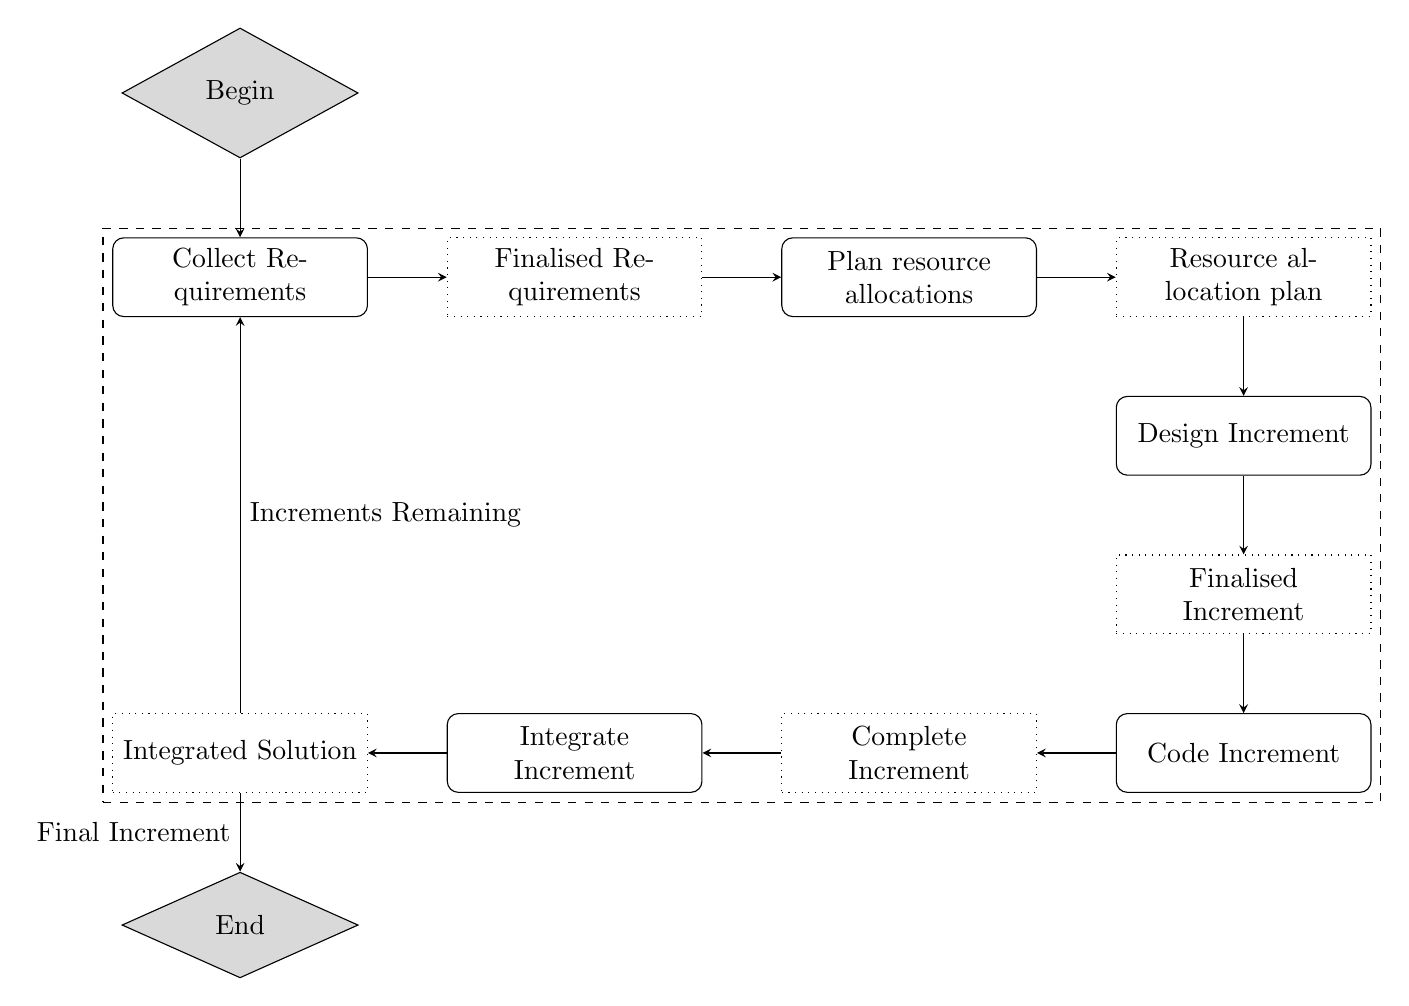
\begin{tikzpicture}[node distance=1cm]
% http://commons.wikimedia.org/wiki/File:Incremental_Model.jpg
\node (start) [startstop] {Begin};


\node (req) [stepa, below=of start] {Collect Requirements};
\node (oreq) [outcome, right=of req] {Finalised Requirements};

\node (plan) [stepa, right=of oreq] {Plan resource allocations};
\node (oplan) [outcome, right=of plan] {Resource allocation plan};

\node (design) [stepa, below=of oplan] {Design Increment};
\node (odesign) [outcome, below=of design] {Finalised Increment};

\node (code) [stepa, below=of odesign] {Code Increment};
\node (ocode) [outcome, left=of code] {Complete Increment};

\node (integrate) [stepa, left=of ocode] {Integrate Increment};
\node (ointegrate) [outcome, left=of integrate] {Integrated Solution};

\node[phase, fit=(req) (oreq) (plan) (oplan) (design) (odesign) (code) (ocode) (integrate) (ointegrate)] {};
 
 
\node (stop) [startstop, below=of ointegrate] {End};


\draw [arrow] (start) -- (req);
\draw [arrow] (req) -- (oreq);
\draw [arrow] (oreq) -- (plan);
\draw [arrow] (plan) -- (oplan);
\draw [arrow] (oplan) -- (design);
\draw [arrow] (design) -- (odesign);
\draw [arrow] (odesign) -- (code);
\draw [arrow] (code) -- (ocode);
\draw [arrow] (ocode) -- (integrate);
\draw [arrow] (integrate) -- (ointegrate);

\draw [arrow] (ointegrate) -- node[anchor=east] {Final Increment} (stop);

\draw [arrow] (ointegrate) -- node[anchor=west] {Increments Remaining} (req);
\end{tikzpicture}



\subsection{Personal Process}
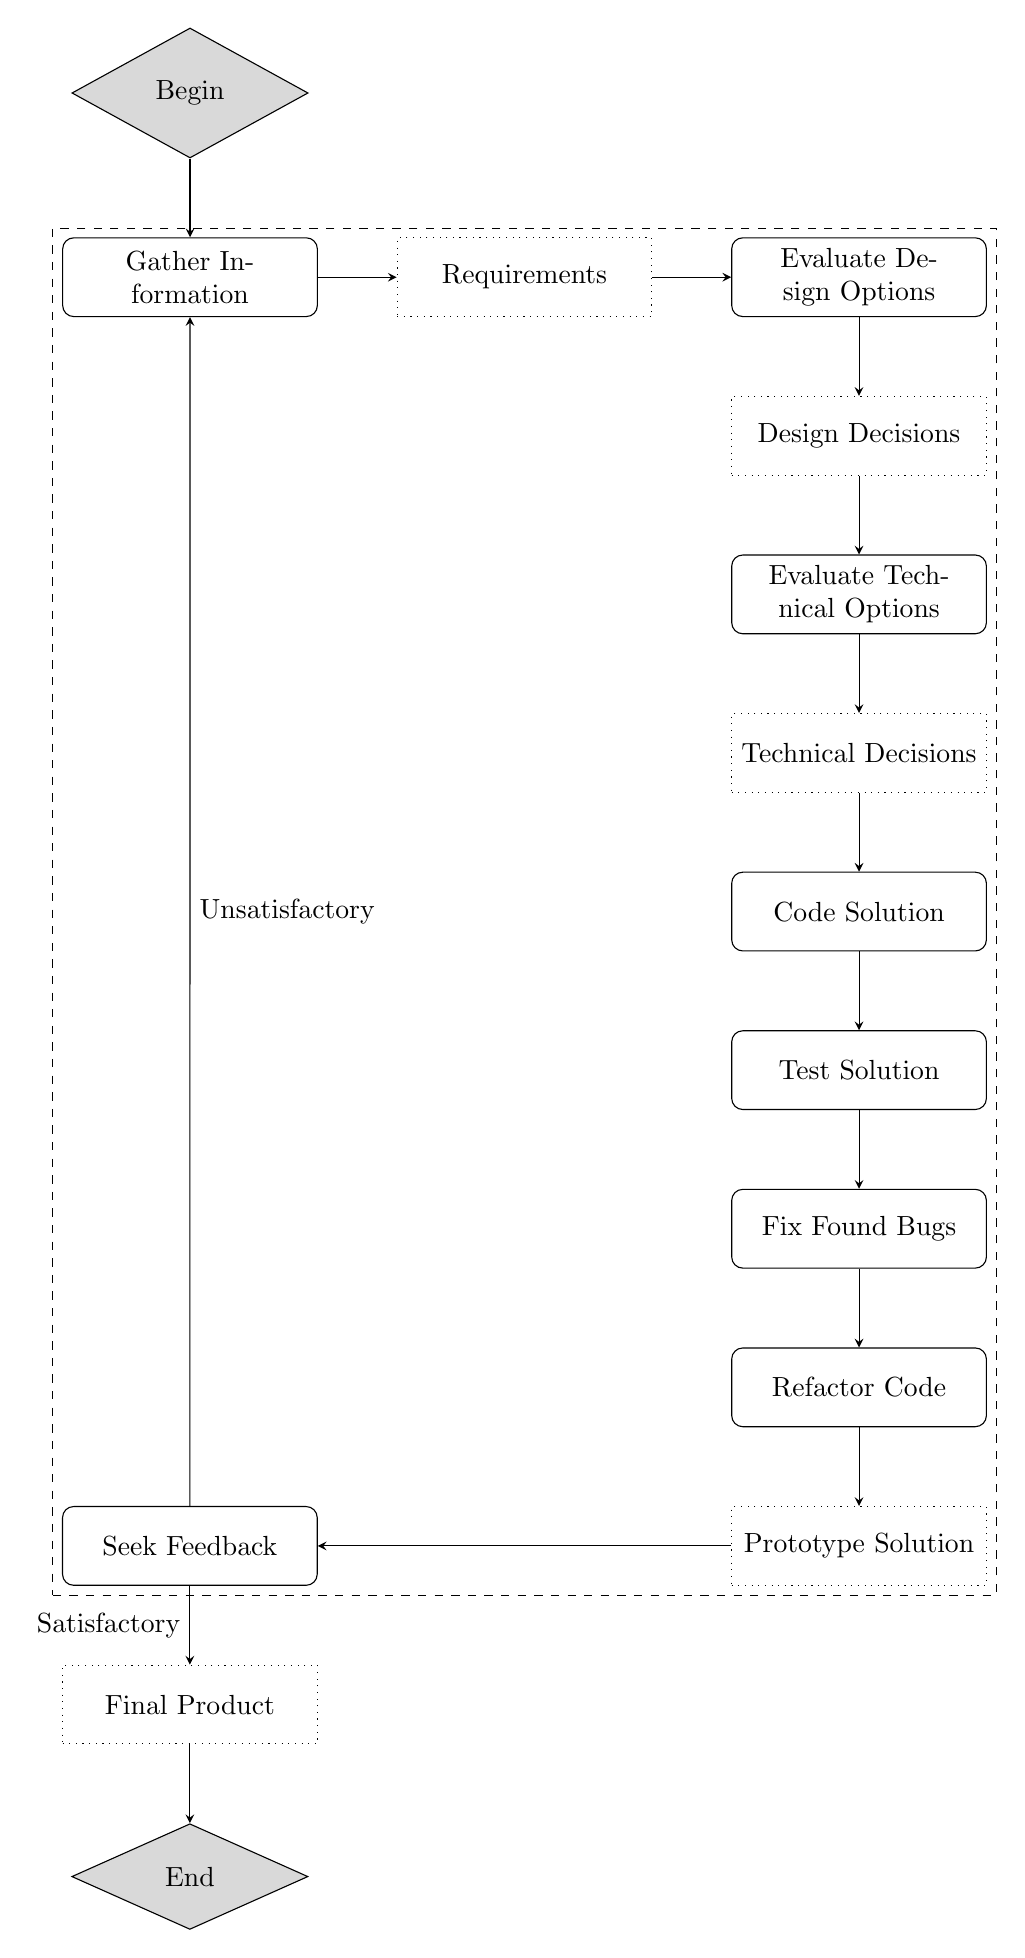
\begin{tikzpicture}[node distance=1cm]

\node (start) [startstop] {Begin};

\node (gather) [stepa, below=of start] {Gather Information};
% \node (client) [infosource, below=of gather] {Client};
\node (probdef) [outcome, right=of gather] {Requirements};
\node (eval) [stepa, right=of probdef] {Evaluate Design Options};

\node (designuse) [outcome, below=of eval] {Design Decisions};
\node (tech) [stepa, below=of designuse] {Evaluate Technical Options};
% \node (internet) [infosource, left=of tech] {Internet};
\node (techuse) [outcome, below=of tech] {Technical Decisions};


\node (code) [stepa, below=of techuse] {Code Solution};
\node (test) [stepa, below=of code] {Test Solution};
\node (bugfix) [stepa, below=of test] {Fix Found Bugs};
\node (refactor) [stepa, below=of bugfix] {Refactor Code};
\node (prototype) [outcome, below=of refactor] {Prototype Solution};
\node (feedback) [stepa, left=5.25cm of prototype] {Seek Feedback};


\node[phase, fit=(gather) (code) (test) (bugfix) (refactor) (prototype) (feedback)] {};

\node (final) [outcome, below=of feedback] {Final Product};
\node (stop) [startstop, below=of final] {End};


% \draw [arrow] (client) -- (gather);
% \draw [arrow] (client) -- (eval);
% \draw [arrow] (client) -- (feedback);

% \draw [arrow] (internet) -- (tech);

\draw [arrow] (start) -- (gather);
\draw [arrow] (gather) -- (probdef);
\draw [arrow] (probdef) -- (eval);
\draw [arrow] (eval) -- (designuse);
\draw [arrow] (designuse) -- (tech);
\draw [arrow] (tech) -- (techuse);
\draw [arrow] (techuse) -- (code);
\draw [arrow] (code) -- (test);
\draw [arrow] (test) -- (bugfix);
\draw [arrow] (bugfix) -- (refactor);
\draw [arrow] (refactor) -- (prototype);
\draw [arrow] (prototype) -- (feedback);
\draw [arrow] (feedback) -- node[anchor=east] {Satisfactory} (final);
\draw [arrow] (feedback) -- node[anchor=west] {Unsatisfactory} (gather);
\draw [arrow] (final) -- (stop);

\end{tikzpicture}


\subsection{Systems Development Life Cycle}
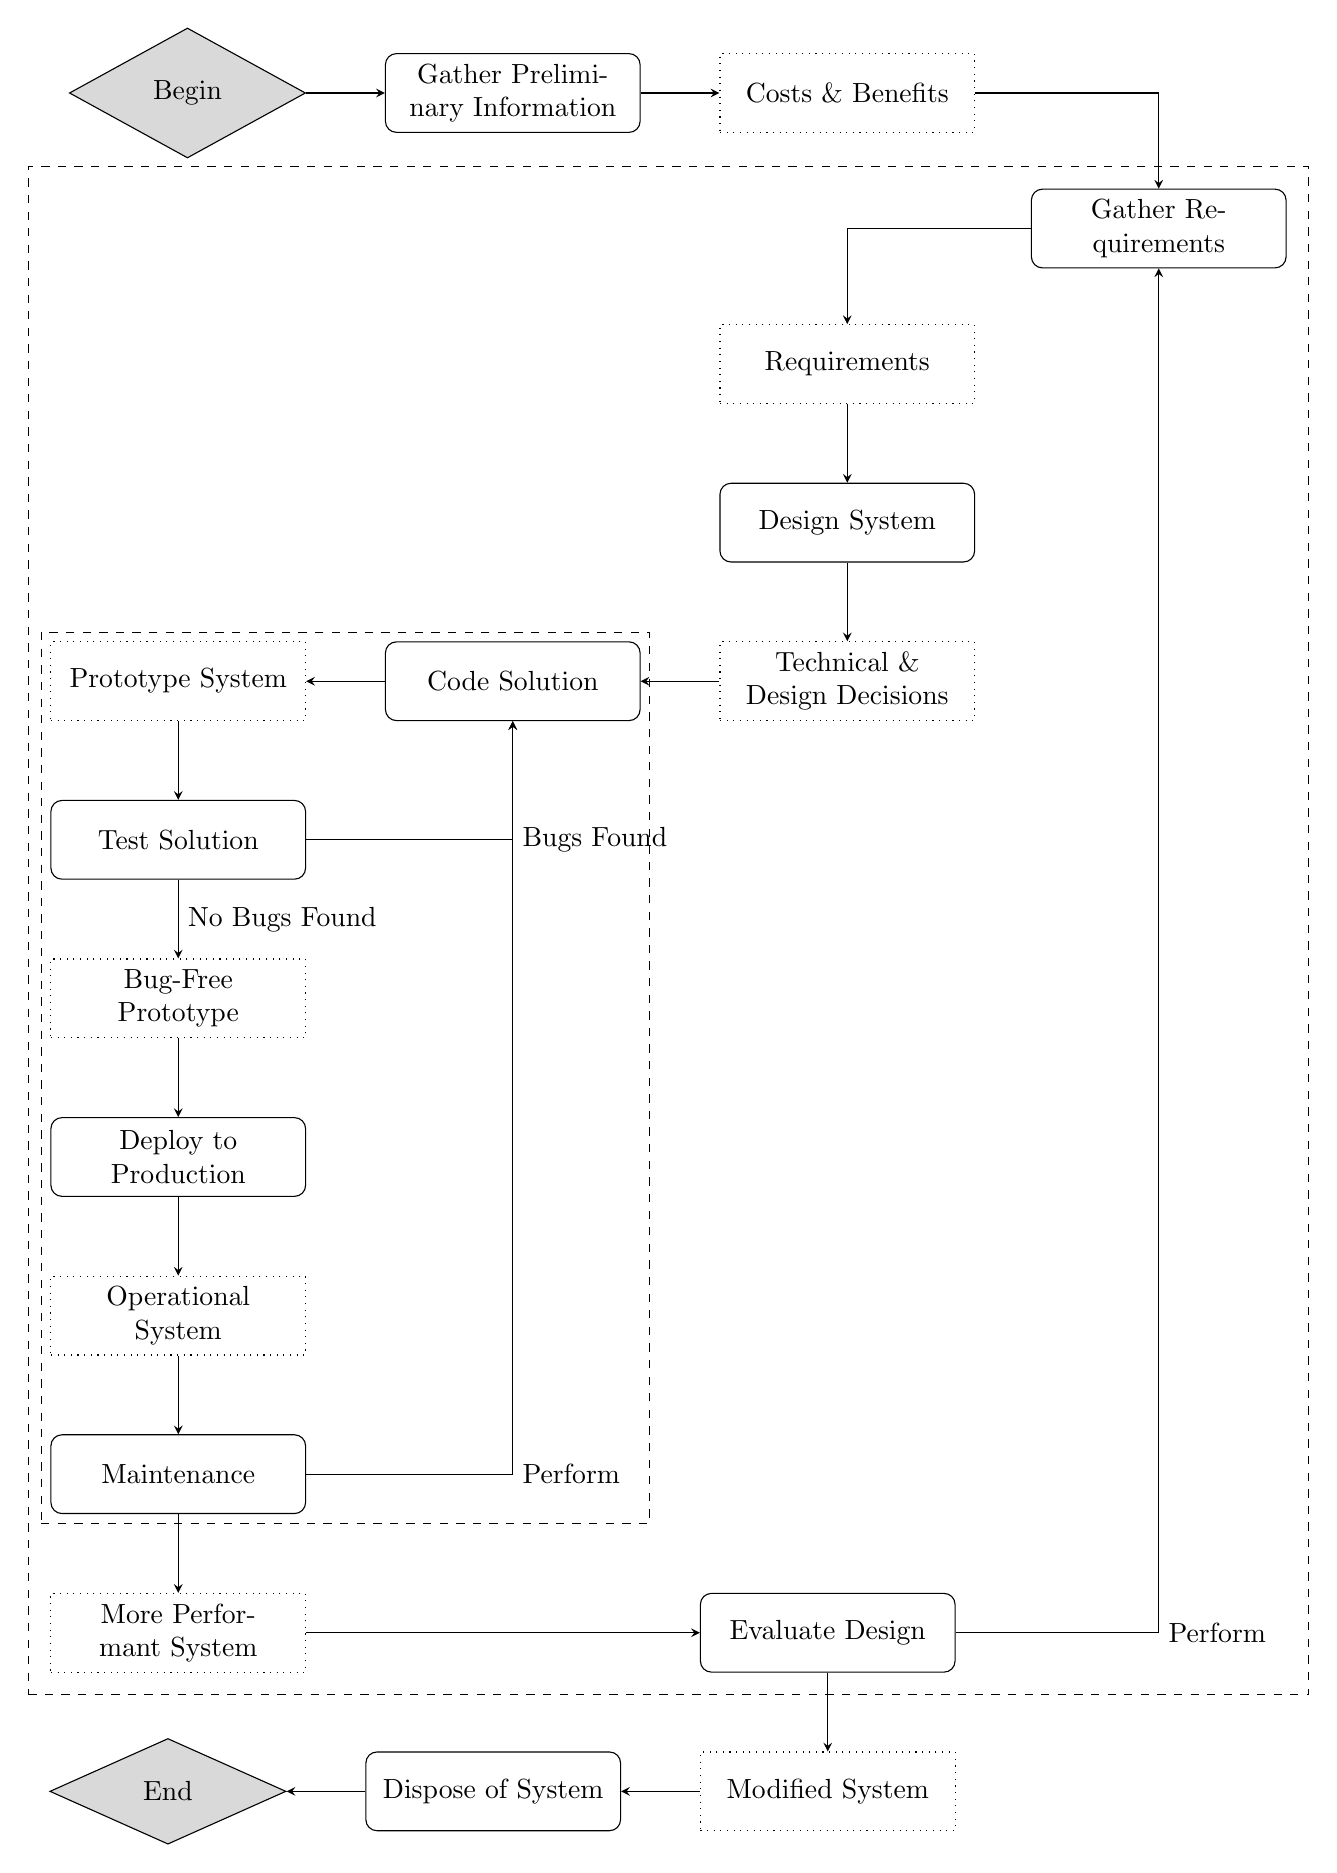
\begin{tikzpicture}[node distance=1cm]
% http://en.wikipedia.org/wiki/Systems_development_life_cycle#Phases
\node (start) [startstop] {Begin};

\node (prelim) [stepa, right=of start] {Gather Preliminary Information};
% \node (stakeholder) [infosource, below=of gather] {Stakeholders};

% \draw [arrow] (stakeholder) -- (prelim);
\draw [arrow] (start) -- (prelim);

\node (costbenefit) [outcome, right=of prelim] {Costs \& Benefits};

\draw [arrow] (prelim) -- (costbenefit);

\node (gather) [stepa, below right=of costbenefit] {Gather Requirements};
% \node (user) [infosource, below=of costbenefit] {User};

\draw [arrow] (costbenefit) -| (gather);
% \draw [arrow] (user) -- (gather);

\node (reqs) [outcome, below left=of gather] {Requirements};
\node (design) [stepa, below=of reqs] {Design System};
\node (designed) [outcome, below=of design] {Technical \& Design Decisions};

\draw [arrow] (gather) -| (reqs);
\draw [arrow] (reqs) -- (design);
\draw [arrow] (design) -- (designed);

\node (code) [stepa, left=of designed] {Code Solution};
\node (prototype) [outcome, left=of code] {Prototype System};

\draw [arrow] (designed) -- (code);
\draw [arrow] (code) -- (prototype);

\node (test) [stepa, below=of prototype] {Test Solution};

\draw [arrow] (prototype) -- (test);

\node (tested) [outcome, below=of test] {Bug-Free Prototype};

\draw [arrow] (test) -| node[anchor=west] {Bugs Found} (code);
\draw [arrow] (test) -- node[anchor=west] {No Bugs Found} (tested);

\node (product) [stepa, below=of tested] {Deploy to Production};

\draw [arrow] (tested) -- (product);

\node (configed) [outcome, below=of product] {Operational System};

\draw [arrow] (product) -- (configed);

\node (maintain) [stepa, below=of configed] {Maintenance};

\draw [arrow] (configed) -- (maintain);

\node (improve) [outcome, below=of maintain] {More Performant System};

\draw [arrow] (maintain) -| node[anchor=west] {Perform} (code);
\draw [arrow] (maintain) -- (improve);

\node (eval) [stepa, right=5cm of improve] {Evaluate Design};

\draw [arrow] (improve) -- (eval);

\node (evalo) [outcome, below=of eval] {Modified System};

\draw [arrow] (eval) -- (evalo);
\draw [arrow] (eval.east) -| node[anchor=west] {Perform} (gather);

\node (disposal) [stepa, left=of evalo] {Dispose of System};

\draw [arrow] (evalo) -- (disposal);

\node (stop) [startstop, left=of disposal] {End};

\draw [arrow] (disposal) -- (stop);


\node[phase, fit=(code) (prototype) (test) (tested) (product) (configed) (maintain)] {};

\node[phase, inner sep=8,fit=(gather) (reqs) (design) (designed) (code) (prototype) (test) (tested) (product) (configed) (maintain) (improve) (eval)] {};


\end{tikzpicture}


\subsection{Spiral Model}
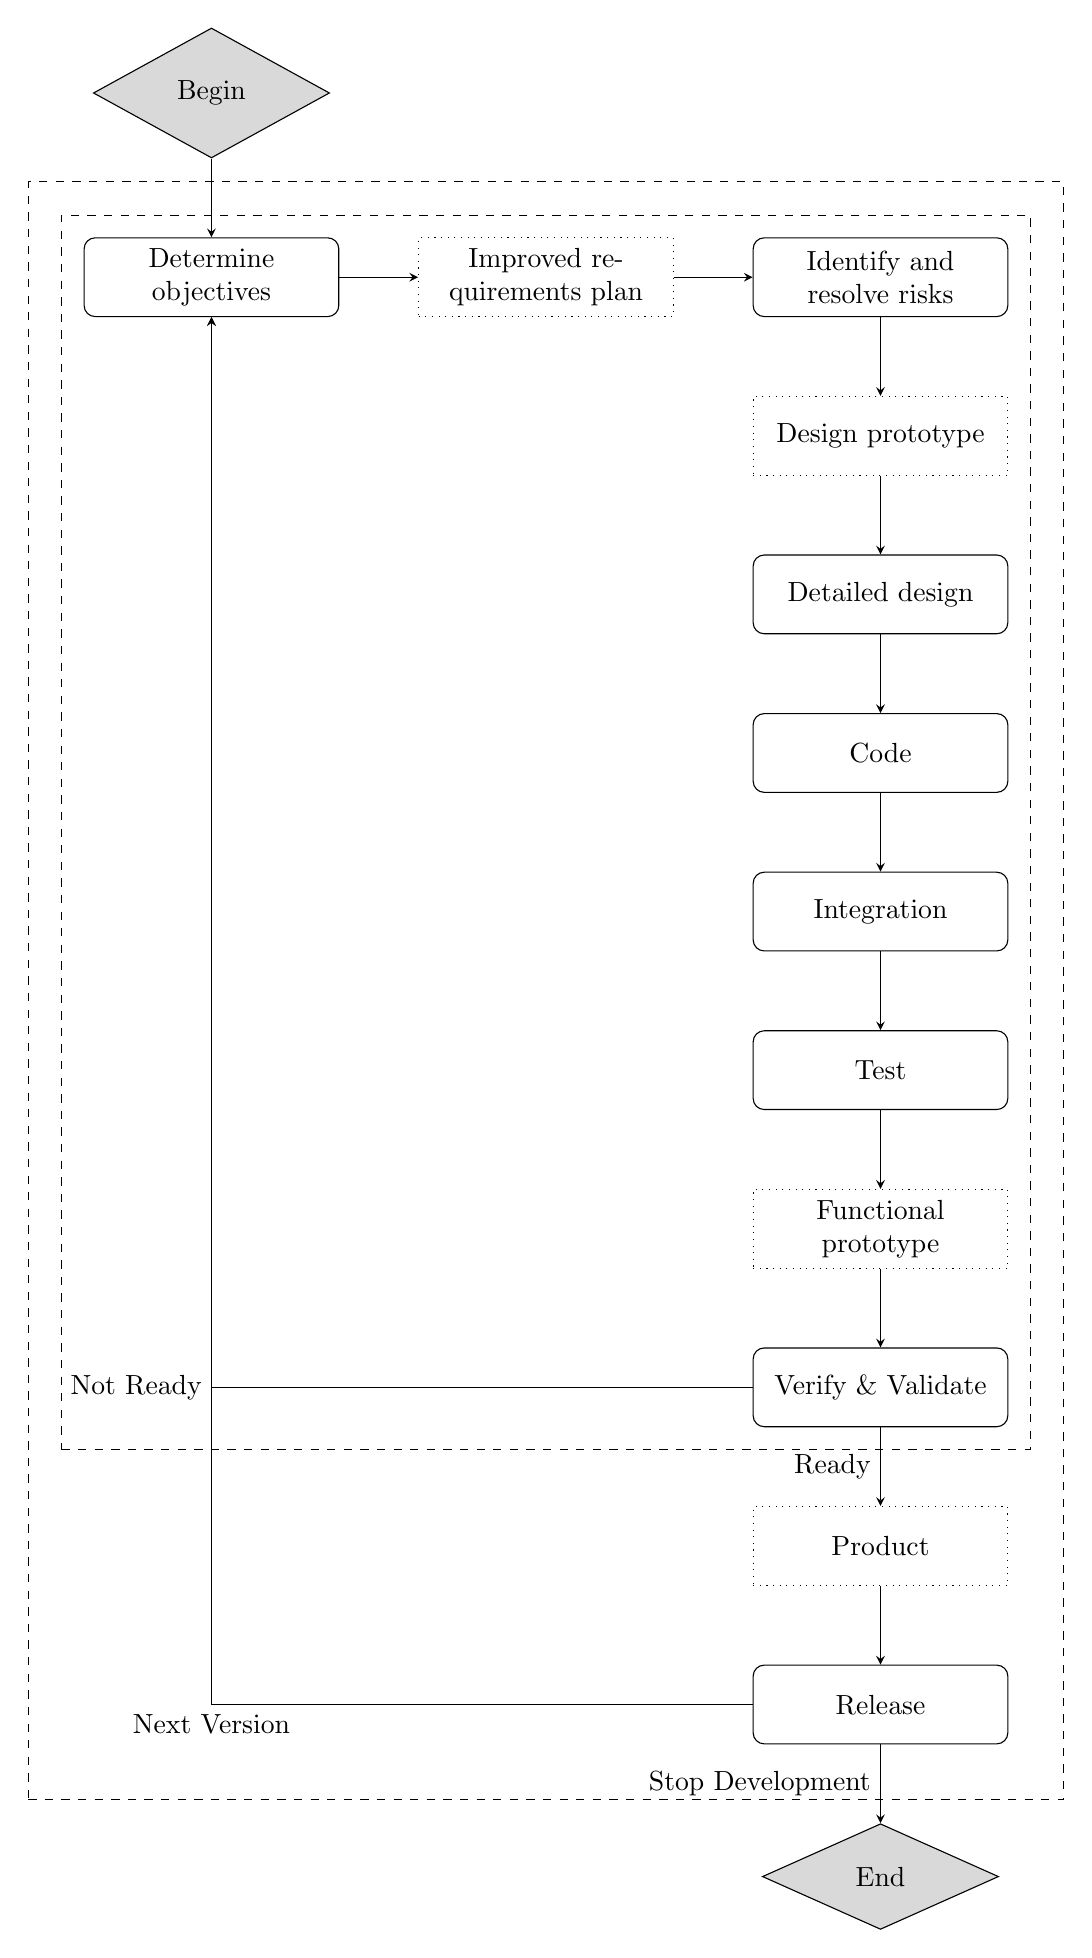
\begin{tikzpicture}[node distance=1cm]
% http://commons.wikimedia.org/wiki/File:Spiral_model_(Boehm,_1988).svg
\node (start) [startstop] {Begin};

\node (prelim) [stepa, below=of start] {Determine objectives};

\node (reqplan) [outcome, right=of prelim] {Improved requirements plan};

\node (risks) [stepa, right=of reqplan] {Identify and resolve risks};

\node (prototype) [outcome, below=of risks] {Design prototype};

\node (design) [stepa, below=of prototype] {Detailed design};
\node (code) [stepa, below=of design] {Code};
\node (integrate) [stepa, below=of code] {Integration};
\node (test) [stepa, below=of integrate] {Test};

\node (prototype2) [outcome, below=of test] {Functional prototype};

\node (verify) [stepa, below=of prototype2] {Verify \& Validate};


\node (product) [outcome, below=of verify] {Product};
\node (release) [stepa, below=of product] {Release};


\node (stop) [startstop, below=of release] {End};


\node[phase, inner sep=20,fit=(prelim) (reqplan) (risks) (prototype) (design) (code) (integrate) (test) (verify) (product) (release)] {};

\node[phase, inner sep=8,fit=(prelim) (reqplan) (risks) (prototype) (design) (code) (integrate) (test) (verify)] {};

\draw [arrow] (start) -- (prelim);
\draw [arrow] (prelim) -- (reqplan);
\draw [arrow] (reqplan) -- (risks);
\draw [arrow] (risks) -- (prototype);
\draw [arrow] (prototype) -- (design);
\draw [arrow] (design) -- (code);
\draw [arrow] (code) -- (integrate);
\draw [arrow] (integrate) -- (test);
\draw [arrow] (test) -- (prototype2);
\draw [arrow] (prototype2) -- (verify);
\draw [arrow] (verify) -- node[anchor=east] {Ready} (product);
\draw [arrow] (product) -- (release);

\draw [arrow] (release) -- node[anchor=east] {Stop Development} (stop);
\draw [arrow] (release) -| node[anchor=north] {Next Version} (prelim);

\draw [arrow] (verify) -| node[anchor=east] {Not Ready} (prelim);
\end{tikzpicture}


\subsection{Agile: Dynamic Systems Development Method}
\label{sec:dsdm}
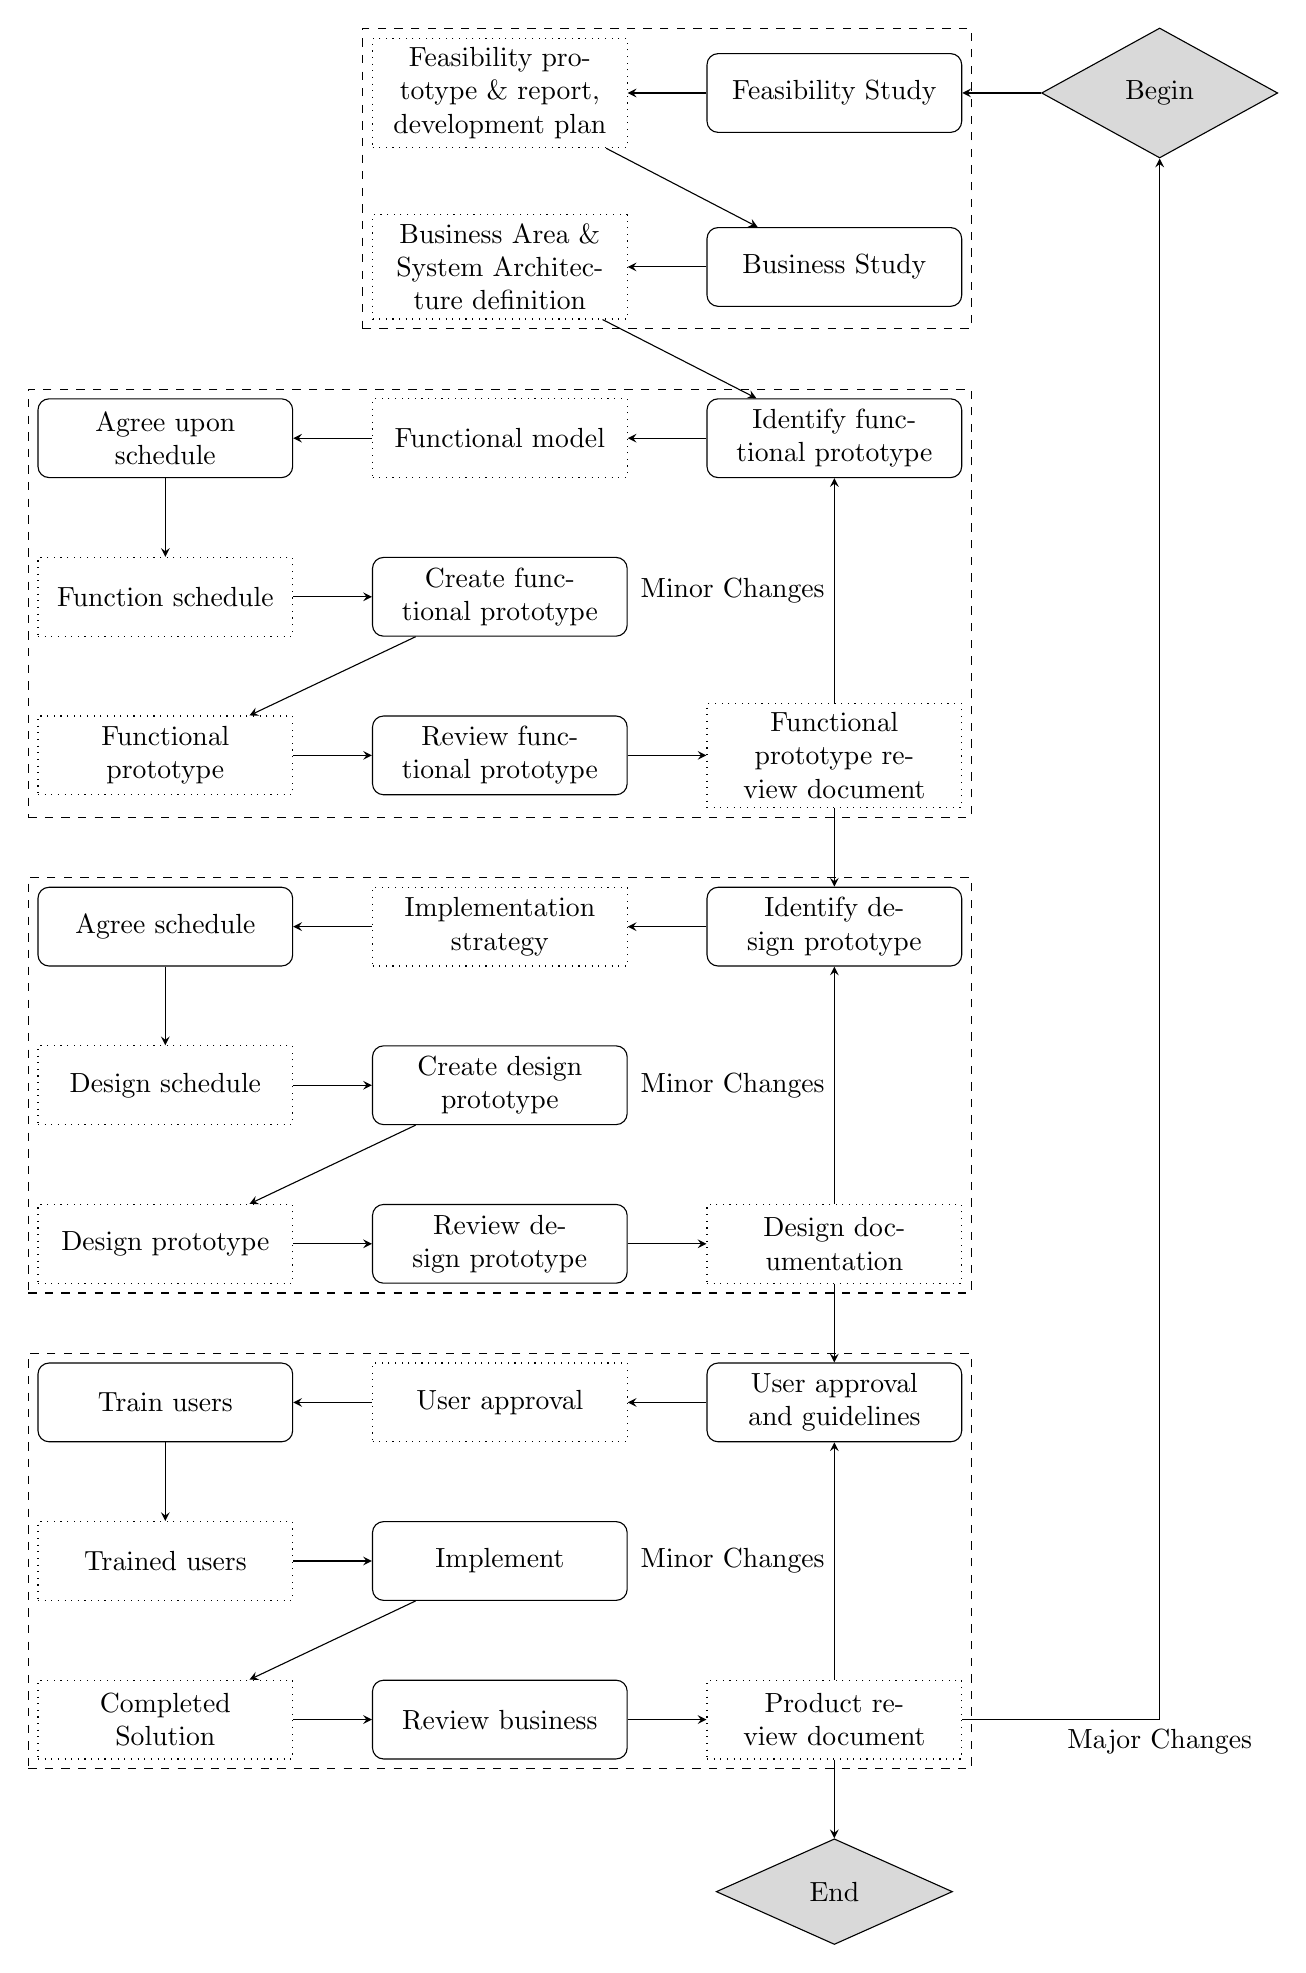
\begin{tikzpicture}[node distance=1cm]
% http://upload.wikimedia.org/wikipedia/commons/f/fb/Processdata-FMI.png
\node (start) [startstop] {Begin};

\node (fstudy) [stepa, left=of start] {Feasibility Study};
\node (fesproto) [outcome, left=of fstudy] {Feasibility prototype \& report, development plan};
\node (bstudy) [stepa, below right=1cm and 1cm of fesproto] {Business Study};
\node (bizproto) [outcome, left=of bstudy] {Business Area \& System Architecture definition};

\node[phase, fit=(fstudy) (fesproto) (bstudy) (bizproto)] {};

\node (fidentify) [stepa, below right=1cm and 1cm of bizproto] {Identify functional prototype};
\node (model) [outcome, left=of fidentify] {Functional model};
\node (fschedule) [stepa, left=of model] {Agree upon schedule};
\node (fsched) [outcome, below=of fschedule] {Function schedule};
\node (fcproto) [stepa, right=of fsched] {Create functional prototype};
\node (fproto) [outcome, below left=1cm and 1cm of fcproto] {Functional prototype};
\node (frproto) [stepa, right=of fproto] {Review functional prototype};
\node (fprotor) [outcome, right=of frproto] {Functional prototype review document};

\node[phase, fit=(fidentify) (model) (fschedule) (fsched) (fcproto) (fproto) (frproto) (fprotor) ] {};

\node (didentify) [stepa, below=of fprotor] {Identify design  prototype};
\node (strats) [outcome, left=of didentify] {Implementation strategy};
\node (dschedule) [stepa, left=of strats] {Agree schedule};
\node (dsched) [outcome, below=of dschedule] {Design schedule};
\node (dcproto) [stepa, right=of dsched] {Create design prototype};
\node (dproto) [outcome, below left=1cm and 1cm of dcproto] {Design prototype};
\node (drproto) [stepa, right=of dproto] {Review design prototype};
\node (ddoc) [outcome, right=of drproto] {Design documentation};

\node[phase, fit=(didentify) (strats) (dschedule) (dsched) (dcproto) (dproto) (drproto) (ddoc)] {}; 

\node (userapp) [stepa, below=of ddoc] {User approval and guidelines};
\node (ouserapp) [outcome, left=of userapp] {User approval};
\node (train) [stepa, left=of ouserapp] {Train users};
\node (otrain) [outcome, below=of train] {Trained users};
\node (implement) [stepa, right=of otrain] {Implement};
\node (system) [outcome,  below left=1cm and 1cm of implement] {Completed Solution};
\node (review) [stepa, right=of system] {Review business};
\node (pr) [outcome, right=of review] {Product review document};

\node[phase, fit=(userapp) (ouserapp) (train) (otrain) (implement) (system) (review) (pr)] {};

\node (end) [startstop, below=of pr] {End};

\draw [arrow] (start) -- (fstudy);

\draw [arrow] (fstudy) -- (fesproto);
\draw [arrow] (fesproto) -- (bstudy);
\draw [arrow] (bstudy) -- (bizproto);

\draw [arrow] (bizproto) -- (fidentify);
\draw [arrow] (fidentify) -- (model);
\draw [arrow] (model) -- (fschedule);
\draw [arrow] (fschedule) -- (fsched);
\draw [arrow] (fsched) -- (fcproto);
\draw [arrow] (fcproto) -- (fproto);
\draw [arrow] (fproto) -- (frproto);
\draw [arrow] (frproto) -- (fprotor);
\draw [arrow] (fprotor) -- (didentify);

\draw [arrow] (fprotor) -- node[anchor=east] {Minor Changes} (fidentify);

\draw [arrow] (didentify) -- (strats);
\draw [arrow] (strats) -- (dschedule);
\draw [arrow] (dschedule) -- (dsched);
\draw [arrow] (dsched) -- (dcproto);
\draw [arrow] (dcproto) -- (dproto);
\draw [arrow] (dproto) -- (drproto);
\draw [arrow] (drproto) -- (ddoc);
\draw [arrow] (ddoc) -- (userapp);

\draw [arrow] (ddoc) -- node[anchor=east] {Minor Changes} (didentify);

\draw [arrow] (userapp) -- (ouserapp);
\draw [arrow] (ouserapp) -- (train);
\draw [arrow] (train) -- (otrain);
\draw [arrow] (otrain) -- (implement);
\draw [arrow] (implement) -- (system);
\draw [arrow] (system) -- (review);
\draw [arrow] (review) -- (pr);

\draw [arrow] (pr) -- node[anchor=east] {Minor Changes} (userapp);

\draw [arrow] (pr) -- (end);

\draw [arrow] (pr) -| node[anchor=north] {Major Changes} (start);
\end{tikzpicture}

\subsection{Agile: Scrum}
\label{sec:scrum}
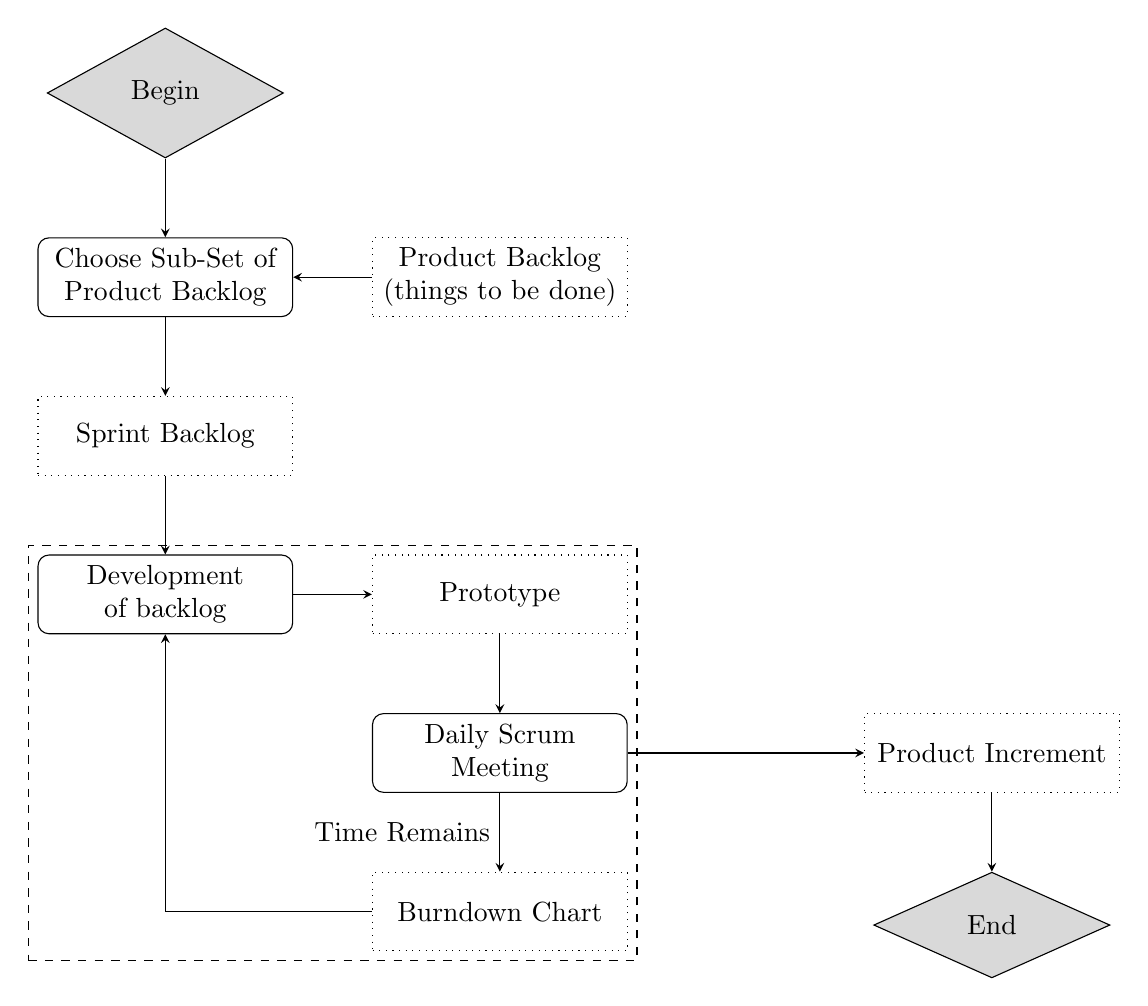
\begin{tikzpicture}[node distance=1cm]
% http://www.mountaingoatsoftware.com/uploads/blog/ScrumMediumLabelled.png

\node (start) [startstop] {Begin};

\node (filter) [stepa, below=of start] {Choose Sub-Set of Product Backlog};
\node (pbacklog) [outcome, right=of filter] {Product Backlog (things to be done)};
\node (sbacklog) [outcome, below=of filter] {Sprint Backlog};

\node (dev) [stepa, below=of sbacklog] {Development of backlog};
\node (proto) [outcome, right=of dev] {Prototype};
\node (meeting) [stepa, below=of proto] {Daily Scrum Meeting};
\node (burndown) [outcome, below=of meeting] {Burndown Chart};

\node (ship) [outcome, right=3cm of meeting] {Product Increment};

\node (end) [startstop, below=of ship] {End};

\node[phase, fit=(dev) (meeting) (burndown)] {};

\draw [arrow] (start) -- (filter);
\draw [arrow] (pbacklog) -- (filter);
\draw [arrow] (filter) -- (sbacklog);
\draw [arrow] (sbacklog) -- (dev);
\draw [arrow] (dev) -- (proto);
\draw [arrow] (proto) -- (meeting);
\draw [arrow] (meeting) -- node[anchor=east] {Time Remains} (burndown);
\draw [arrow] (burndown.west) -| (dev.south);

\draw [arrow] (meeting) -- (ship);

\draw [arrow] (ship) -- (end);

\end{tikzpicture}


\subsection{Iterative Development Model}
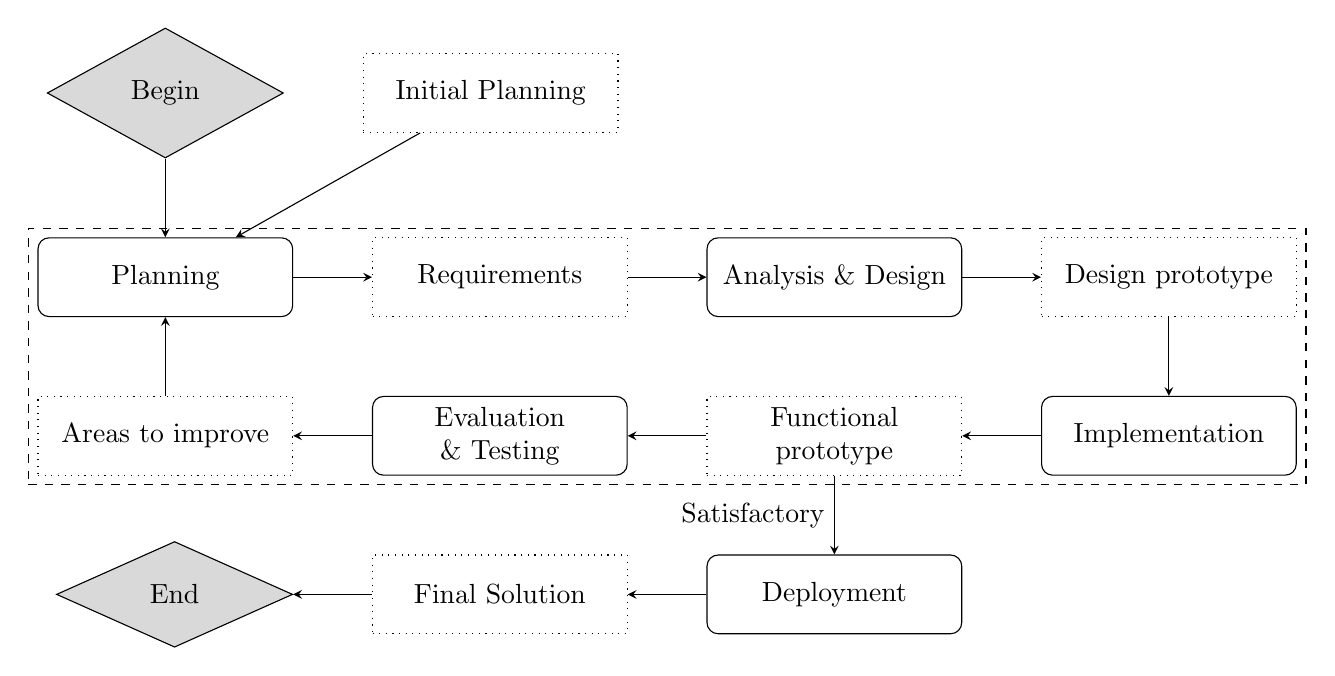
\begin{tikzpicture}[node distance=1cm]
% http://en.wikipedia.org/wiki/File:Iterative_development_model.svg
\node (start) [startstop] {Begin};

\node (init) [outcome, right=of start] {Initial Planning};

\node (plan) [stepa, below=of start] {Planning};
\node (requirements) [outcome, right=of plan] {Requirements};

\node (anal) [stepa, right=of requirements] {Analysis \& Design};
\node (prototype) [outcome, right=of anal] {Design prototype};

\node (implementation) [stepa, below=of prototype] {Implementation};
\node (iproto) [outcome, left=of implementation] {Functional prototype};

\node (testing) [stepa, left=of iproto] {Evaluation \& Testing};
\node (imp) [outcome, left=of testing] {Areas to improve};


\node[phase, fit=(plan) (requirements) (anal) (prototype) (testing) (implementation) (iproto)] {};


\node (deploy) [stepa, below=of iproto] {Deployment};

\node (solution) [outcome, left=of deploy] {Final Solution};
 
\node (end) [startstop, left=of solution] {End};

\draw [arrow] (start) -- (plan);
\draw [arrow] (init) -- (plan);
\draw [arrow] (plan) -- (requirements);
\draw [arrow] (requirements) -- (anal);
\draw [arrow] (anal) -- (prototype);
\draw [arrow] (prototype) -- (implementation);
\draw [arrow] (implementation) -- (iproto);
\draw [arrow] (iproto) -- (testing);
\draw [arrow] (testing) -- (imp);
\draw [arrow] (imp) -- (plan);

\draw [arrow] (iproto) -- node[anchor=east] {Satisfactory} (deploy);
\draw [arrow] (deploy) -- (solution);
\draw [arrow] (solution) -- (end);
\end{tikzpicture}

\subsection{Team Software Process}
\label{sec:tsp}
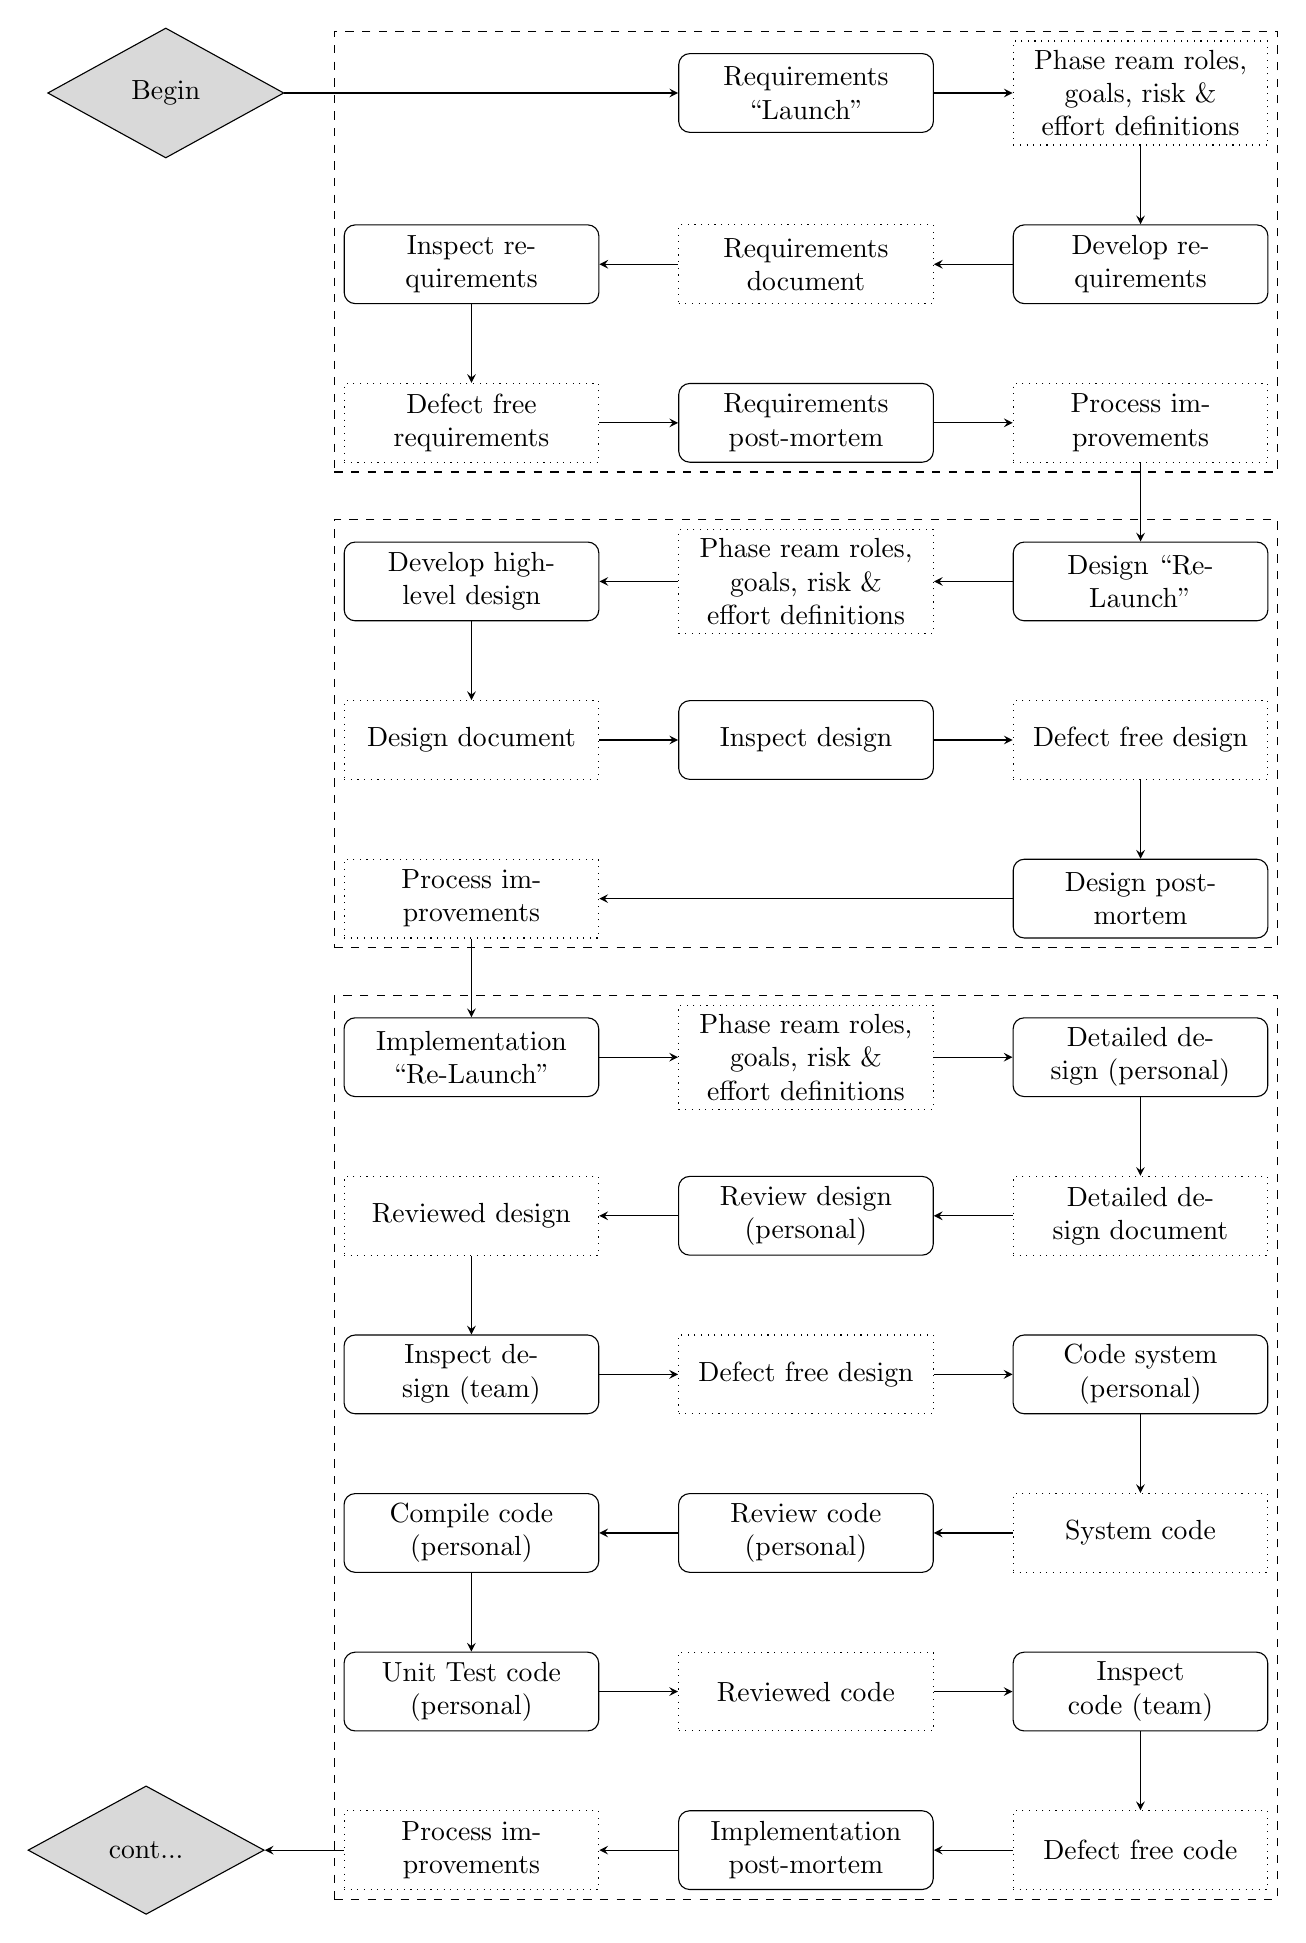
\begin{tikzpicture}[node distance=1cm]
% http://cs.mty.itesm.mx/profesores/pverdines/TCS/p3/PSP-TSP.pdf


\node (start) [startstop] {Begin};

\node (launch1) [stepa, right=5cm of start] {Requirements ``Launch''};
\node (rlaunch1) [outcome, right=of launch1] {Phase ream roles, goals, risk \& effort definitions};

\node (reqs) [stepa, below=of rlaunch1] {Develop requirements};
\node (rreqs) [outcome, left=of reqs] {Requirements document};

\node (insp1) [stepa, left=of rreqs] {Inspect requirements};
\node (rinsp1) [outcome, below=of insp1] {Defect free requirements};

\node (pm1) [stepa, right=of rinsp1] {Requirements post-mortem};
\node (rpm1) [outcome, right=of pm1] {Process improvements};

\draw [arrow] (start) -- (launch1);
\draw [arrow] (launch1) -- (rlaunch1);
\draw [arrow] (rlaunch1) -- (reqs);
\draw [arrow] (reqs) -- (rreqs);
\draw [arrow] (rreqs) -- (insp1);
\draw [arrow] (insp1) -- (rinsp1);
\draw [arrow] (rinsp1) -- (pm1);
\draw [arrow] (pm1) -- (rpm1);


\node[phase, fit=(launch1) (rlaunch1) (reqs) (rreqs) (insp1) (rinsp1) (pm1) (rpm1)] {};

\node (launch2) [stepa, below=of rpm1] {Design ``Re-Launch''};
\node (rlaunch2) [outcome, left=of launch2] {Phase ream roles, goals, risk \& effort definitions};

\node (des) [stepa, left=of rlaunch2] {Develop high-level design};
\node (rdes) [outcome, below=of des] {Design document};

\node (insp2) [stepa, right=of rdes] {Inspect design};
\node (rinsp2) [outcome, right=of insp2] {Defect free design};

\node (pm2) [stepa, below=of rinsp2] {Design post-mortem};
\node (rpm2) [outcome, left=5.25cm of pm2] {Process improvements};

\draw [arrow] (rpm1) -- (launch2);
\draw [arrow] (launch2) -- (rlaunch2);
\draw [arrow] (rlaunch2) -- (des);
\draw [arrow] (des) -- (rdes);
\draw [arrow] (rdes) -- (insp2);
\draw [arrow] (insp2) -- (rinsp2);
\draw [arrow] (rinsp2) -- (pm2);
\draw [arrow] (pm2) -- (rpm2);

\node[phase, fit=(launch2) (rlaunch2) (des) (rdes) (insp2) (rinsp2) (pm2) (rpm2)] {};


\node (launch3) [stepa, below=of rpm2] {Implementation ``Re-Launch''};
\node (rlaunch3) [outcome, right=of launch3] {Phase ream roles, goals, risk \& effort definitions};

\node (ddes) [stepa, right=of rlaunch3] {Detailed design (personal)};
\node (rddes) [outcome, below=of ddes] {Detailed design document};

\node (pinsp3) [stepa, left=of rddes] {Review design (personal)};
\node (prinsp3) [outcome, left=of pinsp3] {Reviewed design};

\node (insp3) [stepa, below=of prinsp3] {Inspect design (team)};
\node (rinsp3) [outcome, right=of insp3] {Defect free design};

\node (cs) [stepa, right=of rinsp3] {Code system (personal)};
\node (rcs) [outcome, below=of cs] {System code};

\node (rc) [stepa, left=of rcs] {Review code (personal)};
\node (cc) [stepa, left=of rc] {Compile code (personal)};
\node (ut) [stepa, below=of cc] {Unit Test code (personal)};
\node (rrc) [outcome, right=of ut] {Reviewed code};

\node (insp4) [stepa, right=of rrc] {Inspect code (team)};
\node (rinsp4) [outcome, below=of insp4] {Defect free code};

\node (pm3) [stepa, left=of rinsp4] {Implementation post-mortem};
\node (rpm3) [outcome, left=of pm3] {Process improvements};

\node (cont) [startstop, left=of rpm3] {cont...};

\draw [arrow] (rpm2) -- (launch3);
\draw [arrow] (launch3) -- (rlaunch3);
\draw [arrow] (rlaunch3) -- (ddes);
\draw [arrow] (ddes) -- (rddes);
\draw [arrow] (rddes) -- (pinsp3);
\draw [arrow] (pinsp3) -- (prinsp3);
\draw [arrow] (prinsp3) -- (insp3);
\draw [arrow] (insp3) -- (rinsp3);
\draw [arrow] (rinsp3) -- (cs);
\draw [arrow] (cs) -- (rcs);
\draw [arrow] (rcs) -- (rc);
\draw [arrow] (rc) -- (cc);
\draw [arrow] (cc) -- (ut);
\draw [arrow] (ut) -- (rrc);
\draw [arrow] (rrc) -- (insp4);
\draw [arrow] (insp4) -- (rinsp4);
\draw [arrow] (rinsp4) -- (pm3);
\draw [arrow] (pm3) -- (rpm3);
\draw [arrow] (rpm3) -- (cont);

\node[phase, fit=(launch3) (rlaunch3) (ddes) (rddes) (pinsp3) (prinsp3) (insp3) (rinsp3) (cs) (rcs) (rc) (cc) (ut) (rrc) (insp4) (rinsp4) (pm3) (rpm3)] {};


\end{tikzpicture}

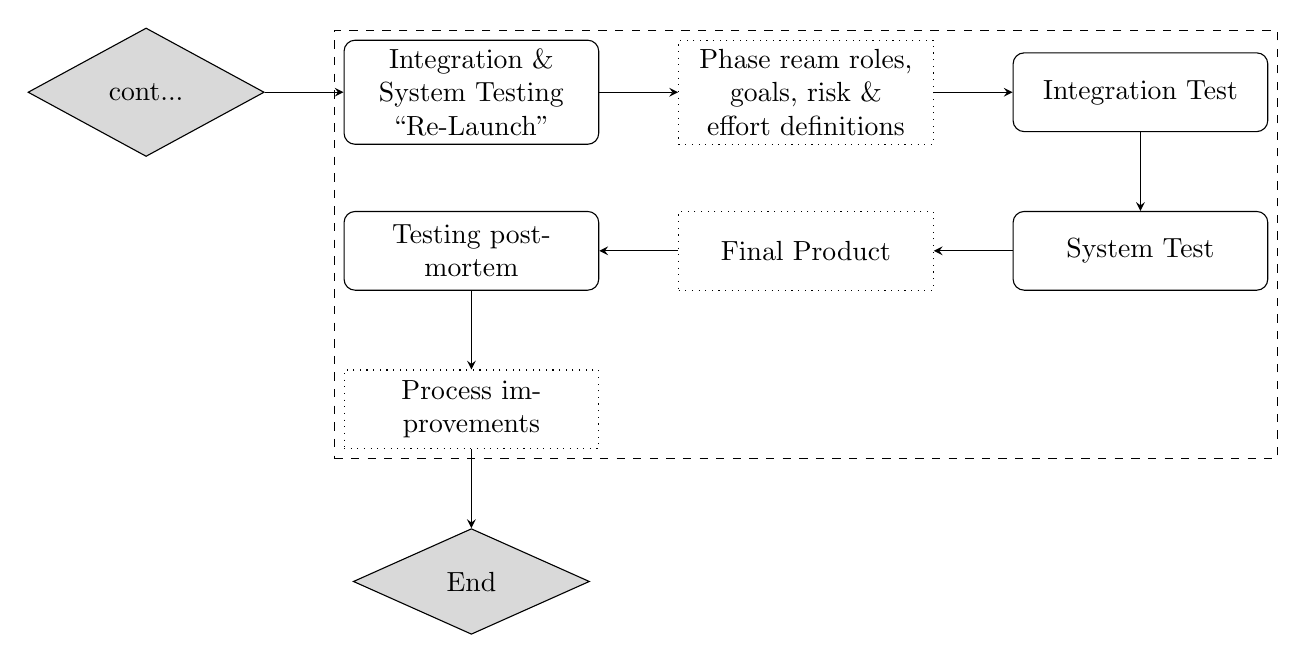
\begin{tikzpicture}[node distance=1cm]
\node (cont) [startstop] {cont...};

\node (launch2) [stepa, right=of cont] {Integration \& System Testing ``Re-Launch''};
\node (rlaunch2) [outcome, right=of launch2] {Phase ream roles, goals, risk \& effort definitions};

\node (des1) [stepa, right=of rlaunch2] {Integration Test};
\node (des2) [stepa, below=of des1] {System Test};
\node (rdes) [outcome, left=of des2] {Final Product};

\node (pm2) [stepa, left=of rdes] {Testing post-mortem};
\node (rpm2) [outcome, below=of pm2] {Process improvements};

\node (stop) [startstop, below=of rpm2] {End};


\draw [arrow] (cont) -- (launch2);
\draw [arrow] (launch2) -- (rlaunch2);
\draw [arrow] (rlaunch2) -- (des1);
\draw [arrow] (des1) -- (des2);
\draw [arrow] (des2) -- (rdes);
\draw [arrow] (rdes) -- (pm2);
\draw [arrow] (pm2) -- (rpm2);
\draw [arrow] (rpm2) -- (stop);

\node[phase, fit=(launch2) (rlaunch2) (des1) (des2) (rdes) (pm2) (rpm2) ] {};
\end{tikzpicture}

\subsection{Feature Driven Development}
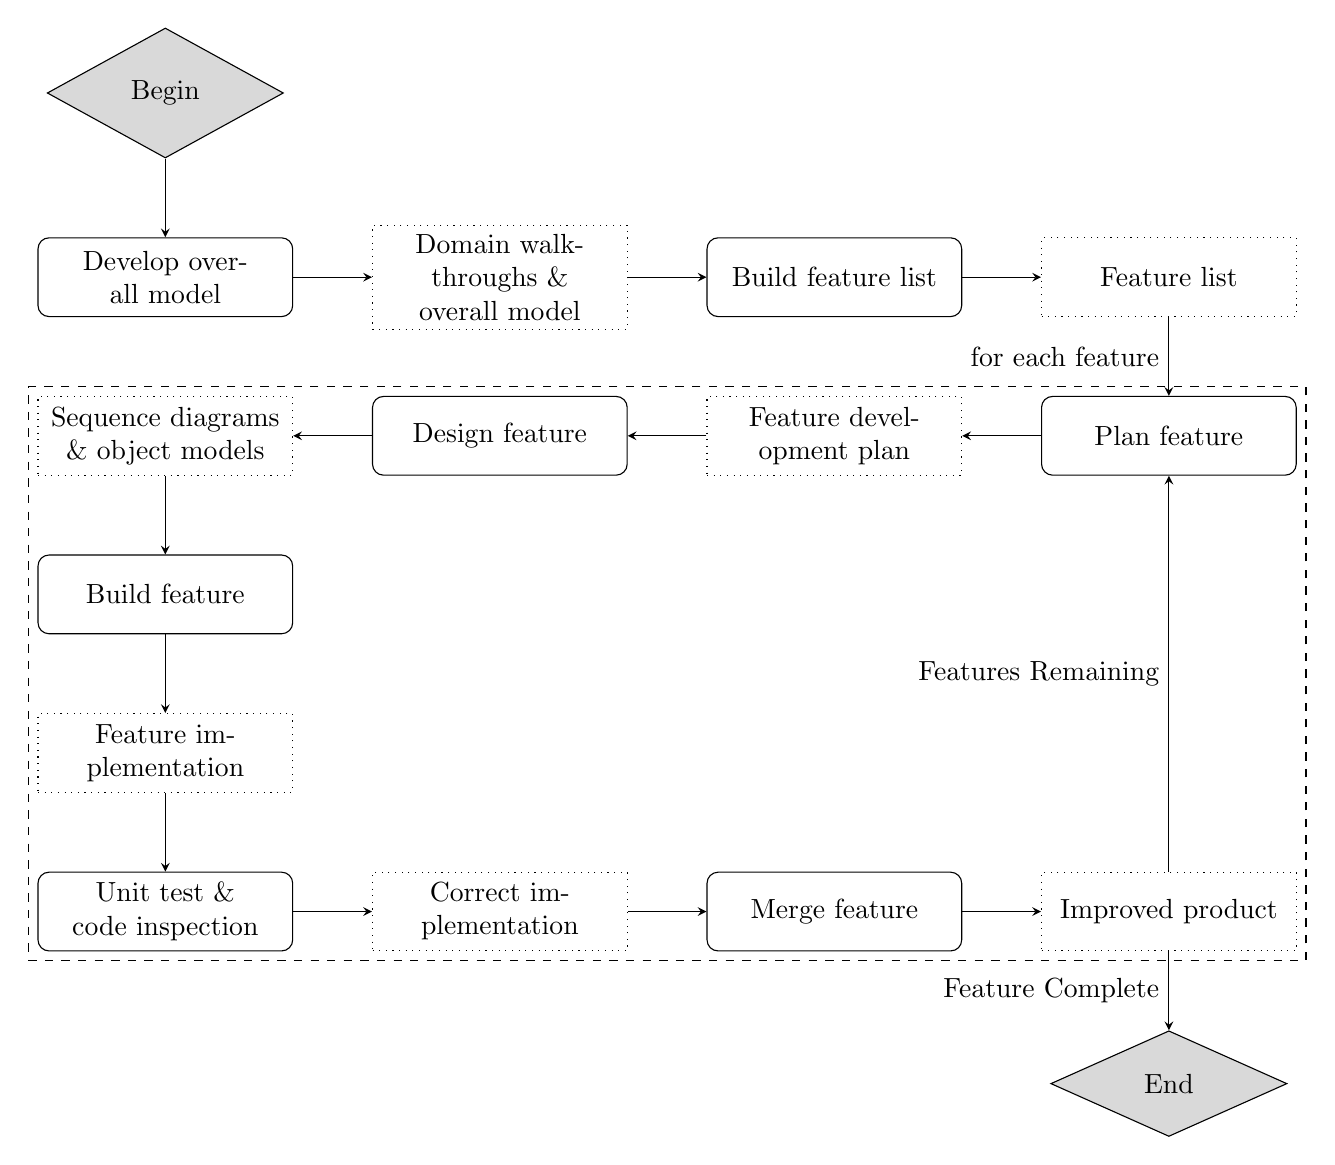
\begin{tikzpicture}[node distance=1cm]
% http://en.wikipedia.org/wiki/Feature_Driven_Development
\node (start) [startstop] {Begin};


\node (req) [stepa, below=of start] {Develop overall model};
\node (oreq) [outcome, right=of req] {Domain walkthroughs \& overall model};

\node (plan) [stepa, right=of oreq] {Build feature list};
\node (oplan) [outcome, right=of plan] {Feature list};

\node (design) [stepa, below=of oplan] {Plan feature};
\node (odesign) [outcome, left=of design] {Feature development plan};

\node (code) [stepa, left=of odesign] {Design feature};
\node (ocode) [outcome, left=of code] {Sequence diagrams \& object models};

\node (integrate) [stepa, below=of ocode] {Build feature};
\node (ointegrate) [outcome, below=of integrate] {Feature implementation};

\node (ut) [stepa, below=of ointegrate] {Unit test \& code inspection};
\node (out) [outcome, right=of ut] {Correct implementation};

\node (m) [stepa, right=of out] {Merge feature};
\node (om) [outcome, right=of m] {Improved product};

\node[phase, fit=(design) (odesign) (code) (ocode) (integrate) (ointegrate) (ut) (out) (m) (om)] {};
 
 
\node (stop) [startstop, below=of om] {End};


\draw [arrow] (start) -- (req);
\draw [arrow] (req) -- (oreq);
\draw [arrow] (oreq) -- (plan);
\draw [arrow] (plan) -- (oplan);
\draw [arrow] (oplan) -- node[anchor=east] {for each feature} (design);
\draw [arrow] (design) -- (odesign);
\draw [arrow] (odesign) -- (code);
\draw [arrow] (code) -- (ocode);
\draw [arrow] (ocode) -- (integrate);
\draw [arrow] (integrate) -- (ointegrate);
\draw [arrow] (ointegrate) -- (ut);
\draw [arrow] (ut) -- (out);
\draw [arrow] (out) -- (m);
\draw [arrow] (m) -- (om);

\draw [arrow] (om) -- node[anchor=east] {Feature Complete} (stop);

\draw [arrow] (om) -- node[anchor=east] {Features Remaining} (design);
\end{tikzpicture}


\subsection{Rational Unified Process}
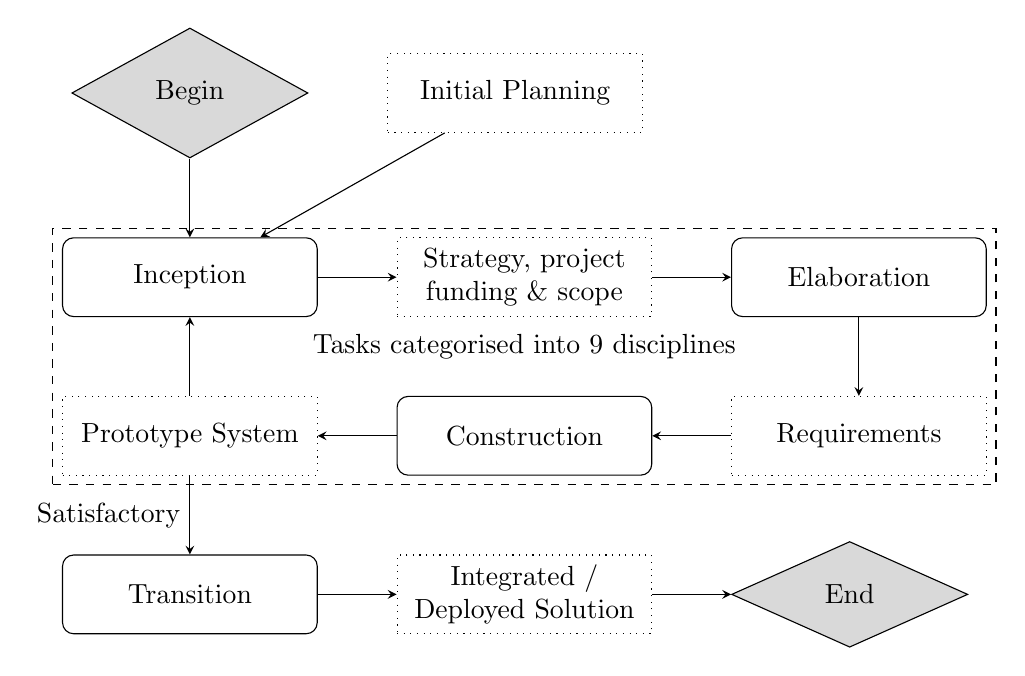
\begin{tikzpicture}[node distance=1cm]
% http://en.wikipedia.org/wiki/File:Iterative_development_model.svg
\node (start) [startstop] {Begin};

\node (init) [outcome, right=of start] {Initial Planning};

\node (ince) [stepa, below=of start] {Inception};

\node (bizstrats) [outcome, right=of ince] {Strategy, project funding \& scope};

\node (plan) [stepa, right=of bizstrats] {Elaboration};
\node (requirements) [outcome, below=of plan] {Requirements};

\node (anal) [stepa, left=of requirements] {Construction};
\node (prototype) [outcome, left=of anal] {Prototype System};


\node[phase, fit=(ince) (bizstrats) (plan) (requirements) (anal) (prototype) ] {Tasks categorised into 9 disciplines};

\node (deploy) [stepa, below=of prototype] {Transition};

\node (solution) [outcome, right=of deploy] {Integrated / Deployed Solution};
 
\node (end) [startstop, right=of solution] {End};

\draw [arrow] (start) -- (ince);
\draw [arrow] (init) -- (ince);
\draw [arrow] (ince) -- (bizstrats);
\draw [arrow] (bizstrats) -- (plan);
\draw [arrow] (plan) -- (requirements);
\draw [arrow] (requirements) -- (anal);
\draw [arrow] (anal) -- (prototype);
\draw [arrow] (prototype) -- (ince);

\draw [arrow] (prototype) -- node[anchor=east] {Satisfactory} (deploy);
\draw [arrow] (deploy) -- (solution);
\draw [arrow] (solution) -- (end);
\end{tikzpicture}


\subsection{Agile Unified Process}
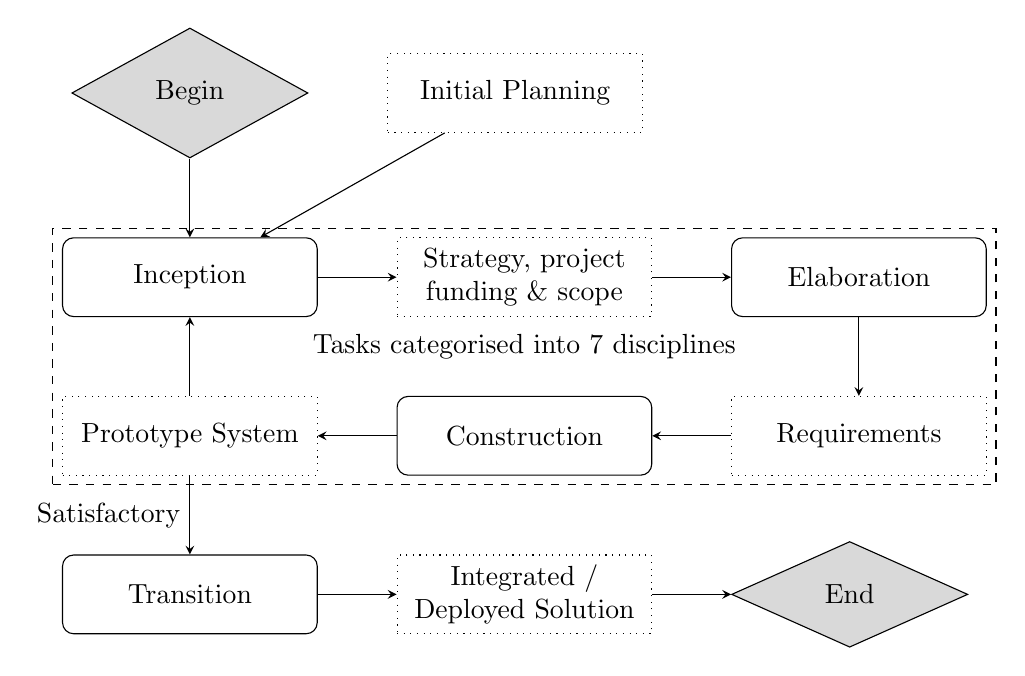
\begin{tikzpicture}[node distance=1cm]
% http://en.wikipedia.org/wiki/Agile_Unified_Process
\node (start) [startstop] {Begin};

\node (init) [outcome, right=of start] {Initial Planning};

\node (ince) [stepa, below=of start] {Inception};

\node (bizstrats) [outcome, right=of ince] {Strategy, project funding \& scope};

\node (plan) [stepa, right=of bizstrats] {Elaboration};
\node (requirements) [outcome, below=of plan] {Requirements};

\node (anal) [stepa, left=of requirements] {Construction};
\node (prototype) [outcome, left=of anal] {Prototype System};


\node[phase, fit=(ince) (bizstrats) (plan) (requirements) (anal) (prototype) ] {Tasks categorised into 7 disciplines};

\node (deploy) [stepa, below=of prototype] {Transition};

\node (solution) [outcome, right=of deploy] {Integrated / Deployed Solution};
 
\node (end) [startstop, right=of solution] {End};

\draw [arrow] (start) -- (ince);
\draw [arrow] (init) -- (ince);
\draw [arrow] (ince) -- (bizstrats);
\draw [arrow] (bizstrats) -- (plan);
\draw [arrow] (plan) -- (requirements);
\draw [arrow] (requirements) -- (anal);
\draw [arrow] (anal) -- (prototype);
\draw [arrow] (prototype) -- (ince);

\draw [arrow] (prototype) -- node[anchor=east] {Satisfactory} (deploy);
\draw [arrow] (deploy) -- (solution);
\draw [arrow] (solution) -- (end);
\end{tikzpicture}


\section{Taxonomy}
\label{sec:tax}
\begin{forest}
for tree={
  grow=0,
  rotate=90
}
[Are requirements reevaluated throughout?
  [Yes
    [Is client feedback or acceptance part of evaluation?,text width=5cm
      [Yes
	[Are there separate feature and design prototypes?,text width=5cm
	  [Yes
	    [Are the scheduling and review emphasised in each stage?,text width=5cm
	      [Yes[Dynamic Systems Development Model,rotate=270]]
	      [No[Iterative Development Model,rotate=270]]
	    ]
	  ]
	  [No
	    [Is deployment or release part of the process?,text width=5cm
	      [Yes
		[Are requirements and analysis \& design included as disciplines?,text width=5cm
		  [Yes[Rational Unified Process,rotate=270]]
		  [No[Agile Unified Process,rotate=270]]
		]
	      ]
	      [No[Personal Process,rotate=270]]
	    ]
	  ]
	]
      ]
      [No
	[Is deployment or release part of the process?,text width=5cm
	  [Yes
	    [Is the software developed in increments?,text width=5cm
	      [Yes[Incremental Build Model,rotate=270]]
	      [No[Spiral Model,rotate=270]]
	    ]
	  ]
	  [No[Scrum,rotate=270]]
	]
      ]
    ]
  ]
  [No
    [Is the software developed in independent chunks?,text width=5cm
      [Yes[Feature Driven Development,rotate=270]]
      [No
	[Is the process' effectiveness reevaluated at each step?,text width=5cm
	  [Yes[Team Software Process,rotate=270]]
	  [No[Systems Development Life Cycle,rotate=270]]
        ]
      ]
    ]
  ]
]
\end{forest}

\clearpage
\newgeometry{margin=3.5cm}
\begin{thebibliography}{9}
\bibitem{inc} Incremental Build Model, \url{http://www.technotrice.com/incremental-model-in-software-engineering/}, Accessed: \today

\bibitem{sdlc} Systems Develop Life Cycle, \url{http://www.computerworld.com/s/article/71151/System_Development_Life_Cycle}, Accessed: \today

\bibitem{spiral} Spiral Model, \url{http://commons.wikimedia.org/wiki/File:Spiral_model_(Boehm,_1988).svg}, Accessed: \today

\bibitem{dsdm} Dynamic Systems Development Method, \url{http://commons.wikimedia.org/wiki/File:Processdata-FMI.png}, Accessed: \today

\bibitem{scrum} Scrum, \url{http://www.mountaingoatsoftware.com/uploads/blog/ScrumMediumLabelled.png}, Accessed: \today

\bibitem{iter} Iterative Development Model, \url{http://commons.wikimedia.org/wiki/File:Iterative_development_model.svg}, Accessed: \today

\bibitem{tsp} Team Software Process, Page 33, \url{http://cs.mty.itesm.mx/profesores/pverdines/TCS/p3/PSP-TSP.pdf}, Accessed: \today

\bibitem{fdd} Feature Driven Development, \url{http://commons.wikimedia.org/wiki/File:Fdd_process_diagram.png}, Accessed: \today

\bibitem{rup} Rational Unified Process, \url{http://projects.staffs.ac.uk/suniwe/project/projectapproach.html}, Accessed: \today

\bibitem{aup} Agile Unified Process, \url{http://www.ambysoft.com/unifiedprocess/agileUP.html}, Accessed: \today
\end{thebibliography}
\restoregeometry

\clearpage
\begin{appendices}
 \section{Personal Process Program}
 
 \subsection{Source Code}
 \begin{lstlisting}
# Written in Python 3.3
from decimal import *
from math import radians
import itertools

# In degrees
PLACES = {
  'uwa':        ('-31.981179', '115.81991'),
  'perth':      ('-31.954265', '115.8523935'),
  'greenwich':  ('51.4825766', '-0.0076589'),
  'southpole':  ('-85', '0'),
}

RADIUS_EARTH = 6378


# Uses the Haversine formula
# Assumes spherical earth and radian coordinates
def distance(coord1, coord2):
  from math import asin, sqrt, cos, sin

  (lat1, long1), (lat2, long2) = coord1, coord2

  def haversin(v):
    return (sin(v/2))**2

  return 2 * RADIUS_EARTH * asin(
      sqrt(
        haversin(lat2 - lat1) + 
        cos(lat1) * cos(lat2) * haversin(long2 - long1)
      )
    )


if __name__ == '__main__':
  # Convert string coords into Decimal radian objects
  conv_places = {
    x : ( radians(Decimal(y1)), radians(Decimal(y2)) ) 
    for x, (y1, y2) in PLACES.items()
  }

  print('Distance calculations!')
  print()

  # Iterate over all place combinations and print the answers
  for (n1, c1), (n2, c2) in itertools.combinations(conv_places.items(), 2):

    print('Distance from {} to {}'.format(n1, n2))
    print('  = {}'.format(distance(c1, c2)))
    print()
 \end{lstlisting}

 \newpage
 \subsection{Output}
 \begin{lstlisting}[language= ]
Distance calculations!

Distance from perth to uwa
  = 4.287899604948252

Distance from perth to greenwich
  = 14485.978495782614

Distance from perth to southpole
  = 6715.917481245382

Distance from uwa to greenwich
  = 14485.767563601663

Distance from uwa to southpole
  = 6712.656749767587

Distance from greenwich to southpole
  = 15192.844590121906
 \end{lstlisting}

 \subsection{Development Timings}
 Timings have been submitted to lecturer.
 
\end{appendices}


\end{document}
